\section{约束下的选点}
\label{sec:bo-constraints}

前面的搜索域是已知的。实际问题常带约束，其中有两类要分开。已知且容易判断的约束，比如参数上下限、整数限制，在内层问题~\eqref{eq:bo-inner}里直接限定搜索域即可，真实评价都发生在可行点上。另一类是未知且昂贵的约束：例如“峰值应力不超过上限”，只有仿真运行结束才知道是否满足。

设目标损失和性能上限都要运行才能测得，问题写成
\begin{equation}
 \min_{\bm{x}\in\bm{C}}\ f(\bm{x})\quad\text{s.t.}\quad g_j(\bm{x})\leq0,\ \ j=1,\ldots,m.
 \label{eq:bo-constrained}
\end{equation}
一个候选点的目标值可以很好，却是不可行的。怎样让未知约束进入选点，而“最终可行”和“每次试验都可行”又有什么不同？

\subsection{可行概率}
\label{sec:bo-feasibility}

对每个$g_j$也用一个代理建模，得到后验$G_j$。候选点满足全部约束的后验概率称为可行概率。若当前后验下各约束相互独立，并且第$j$个约束的后验为$N(m_j(\bm{x}),s_j^2(\bm{x}))$，$s_j(\bm{x})>0$，则
\begin{equation}
 \mathrm{PF}_t(\bm{x})=\prod_{j=1}^m\Phi\left(\frac{-m_j(\bm{x})}{s_j(\bm{x})}\right).
 \label{eq:bo-feasible-prob}
\end{equation}

阈值$b_t$也要相应改变：它是已评价点中\emph{可行者}的最好读数。一个不可行点读数再低，也不能作为改进的基准。可行改进的期望是
\[
 \mathbb{E}\Bigl[\bigl(b_t-F(\bm{x})\bigr)_+\,\mathbf{1}\{G_j(\bm{x})\leq0,\ \forall j\}\,\Bigm|\,\mathcal{D}_t\Bigr].
\]
其中$\mathbf{1}\{\cdot\}$表示事件成立时取$1$、否则取$0$。

当前后验下，目标改进与各约束事件相互独立时，乘积的期望等于期望的乘积，所以
\begin{equation}
 \mathrm{cEI}_t(\bm{x})=\mathrm{EI}_t(\bm{x})\cdot\mathrm{PF}_t(\bm{x}).
 \label{eq:bo-cei}
\end{equation}
独立这个条件不能省略。若目标和约束由同一个物理量驱动，相关性强，式~\eqref{eq:bo-cei}就不再是可行改进的期望，需要联合积分。

\paragraph{贯穿例}
在贯穿例上加一个约束$g(x)=(x-4.5)/4\leq0$，算法只能通过评价得知它的值，用同样的核建模。三个读数为$g(1)=-0.875$，$g(4)=-0.125$，$g(7)=0.625$。$x=7$不可行，尽管它读数最低，因此可行最好值是
\[
 b_3=f(1)=0.2.
\]

计算$x=2$的$\mathrm{cEI}$。目标的后验$m=0.143$，$s=0.864$，代入式~\eqref{eq:bo-ei}得$\mathrm{EI}\approx0.374$。约束的后验$m_g\approx-0.445$，$s_g\approx0.864$，可行概率为
\[
 \Phi(0.445/0.864)=\Phi(0.515)\approx0.697.
\]
于是
\[
 \mathrm{cEI}(2)\approx0.374\times0.697\approx0.261.
\]

表~\ref{tab:bo-cei}列出几个候选的结果。不考虑约束的EI选择$x=8$，加上可行概率之后，右侧候选的分数大幅下降，最大值转到$x=0$。图~\ref{fig:bo-constrained}画出了完整的曲线：$x=7$的EI是$0.5$，但$g(7)>0$已知，cEI为$0$。

\begin{BookInlineTable}
 \centering
 \caption{贯穿例的约束选点，$t=3$，$b_3=0.2$（可行读数中最小的）。}
 \label{tab:bo-cei}
 \begin{tabular}{cccccc}
 \toprule
 $x$&$\mathrm{EI}$&$m_g$&$s_g$&$\mathrm{PF}$&$\mathrm{cEI}$\\
 \midrule
 0&0.398&$-0.437$&0.866&0.693&$\mathbf{0.276}$\\
 2&0.374&$-0.445$&0.864&0.697&0.261\\
 6&0.520&0.305&0.864&0.362&0.188\\
 8&0.549&0.313&0.866&0.359&0.197\\
 \bottomrule
 \end{tabular}
\end{BookInlineTable}

\begin{BookInlineFigure}
 \centering
 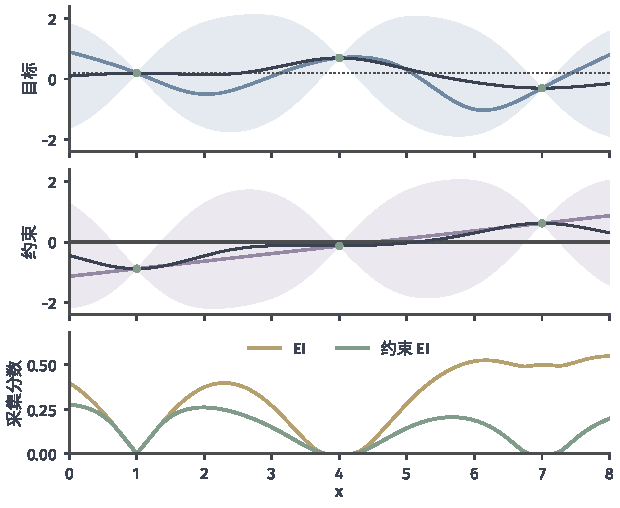
\includegraphics[width=105mm]{figures/05-optimization/05-stochastic-optimization/matplotlib/bo-constrained/figure.pdf}
 \caption{未知约束下的选点。上：目标的后验，蓝线是目标，点线是当前可行最好值$b_3=0.2$。中：约束的后验，紫线是真实的$g$，深灰线是边界$g=0$。下：黄线是不考虑约束的EI，绿线是约束EI，$x=7$处EI较大但已知不可行，约束EI为$0$。}
 \label{fig:bo-constrained}
\end{BookInlineFigure}

\paragraph{还没有可行点时}
读数中若没有可行点，$b_t$没有定义，EI也就无从算起。这时需要先规定一个寻找可行点的准则，最常见的是选$\mathrm{PF}_t(\bm{x})$最大的位置，等找到第一个可行点后，再转入$\mathrm{cEI}$。

\subsection{评价的可行性}
\label{sec:bo-eval-feasibility}

约束有两种含义，到这里还没有分开：一种要求\emph{最终推荐解}可行，中途的试验可以不可行；另一种要求\emph{每次试验}都不能违反约束，比如试验中的设备一旦过热就会损坏。前面的$\mathrm{cEI}$只处理第一种，它会故意到不可行区域采样，以弄清边界。

第二种要求要严格得多。单个点的后验可行概率高并不够用。设每轮选的点可行概率都是$0.95$，假设各轮近似独立，$20$轮全部可行的概率只有
\[
 0.95^{20}\approx0.36.
\]
要保证每次试验都可行，需要三样额外的东西：能把模型与真实约束联系起来的假设（例如$g$确实来自这个高斯过程，或有已知的Lipschitz常数）、至少一个已知可行的初始点、以及保守的选点规则。

图~\ref{fig:bo-safe-set}展示了一种保守的做法：以$g$的后验上界$m_g+2s_g\leq0$定义\emph{安全集}，每轮只在安全集内选点，示例中都取安全集的右端点。这里的约束是前面的$g(x)=(x-4.5)/4$，初始已知$x=1$可行。安全集三轮依次为
\[
 [0.66,1.34],\qquad[0.48,1.76],\qquad[0.32,2.28].
\]
这样的扩张靠边界附近的试验逐步推进，很慢，也可能永远到不了与初始点隔开的另一块可行区域。而且上界中的系数$2$是单点意义上的；要保证所有试验都安全，系数还须按第~\ref{sec:bo-guarantees}节的方式放大。

\begin{BookInlineFigure}
 \centering
 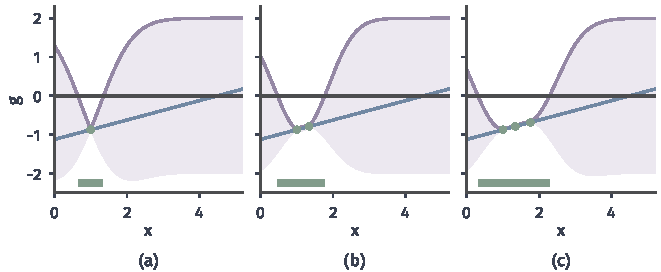
\includegraphics[width=112mm]{figures/05-optimization/05-stochastic-optimization/matplotlib/bo-safe-set/figure.pdf}
 \caption{保守选点下安全集的扩张。蓝线是真实约束$g(x)=(x-4.5)/4$，深灰线是边界，浅紫带是后验$m_g\pm2s_g$，紫线是上界$m_g+2s_g$，绿点是已做的试验，底部绿色粗线是上界不超过$0$的安全集。(a)、(b)、(c)依次是第一、二、三轮。}
 \label{fig:bo-safe-set}
\end{BookInlineFigure}
